\documentclass[11pt, oneside, a4paper]{scrreprt}
\pagestyle{headings}

\usepackage[german, english]{babel}	% 
\usepackage{robocup} 				% Color ifablue for captions
\usepackage{graphicx}				%  \includegraphics
\usepackage[framed]{mcode}			% MATLAB-Code
\usepackage{pst-all,pst-circ}			% PS-Tricks, Electrical circuits
\usepackage{microtype}
%\usepackage{amssymb}
%\usepackage{graphics}
%\usepackage{multicol}
%\usepackage{alltt}

%\usepackage{epsfig}
%\usepackage{amsmath}
%\usepackage{verbatim}

%\usepackage[official]{eurosym}
\usepackage{scrpage2}
%\usepackage{pdfpages}		% Nicht Brauchbar mit PDF





% -  -  -  -  -  -  -  -  -  -  -  -  -  -  -  -  -  -  -  -  -  -  -  -  -  -  -  -  -  -  -  -  -  -  -  -  -  -  -  -  -  -  -  -  -  -  -  -  -  -  -  -  - %
\begin{document}
	\begin{titlepage}
\begin{center}

\begin{figure}[!ht]
\begin{center}
\centerline{ 
\includegraphics[height=16mm]{./Pictures/ethz_logo}
              \hspace{25mm}
%              \includegraphics[height=12mm]{psl_plain}}
	    
\includegraphics[height=12mm]{./Pictures/ifalogo_color}}
\end{center}
\end{figure}

\vspace*{20mm}

{Fabio Marti},
{Matthias Roggo},
{David Lehnen},
{Daniel Gilgen}\\

\vspace{10mm} {\LARGE \bf Robocup: Cooperative estimation and prediction of player and ball movement \\} \vspace{10mm}
{Group Project} \\

\vspace{50mm}

Department: \\
IfA -- Automatic Control Laboratory, ETH Z\"urich \\

\vspace{5mm}
Supervising Professor: \\
Prof.~Dr.~John Lygeros, ETH Z\"urich \\

\vspace{5mm}
Supervisor: \\
M.S., Ph.D. Student Sean Summer, ETH Z\"urich \\

\vspace{10mm}
Z\"urich, March 2012

\end{center}
\end{titlepage}
   		% includes title page.tex
	
\section*{Abstract\markboth{ABSTRACT}{ABSTRACT}} % *: Keine Numerierung des Abschnitts, \markboth: was
% in der Kopfzeile stehen soll

Hier kommt das Abstract ...
      		% includes abstract.tex
	\tableofcontents        	% generates the table of content
	\newpage
	\listoffigures		% generates the table of figures
	% including Sections
	
%-----Chapter 1: Introduction-------%
\chapter{Introduction}

	
%-----Chapter 2: Simulation-------%
\chapter{Simulation}

One main aspect of this group work among the design of a Kalman filter was the construction of a graphical environment for our work, so we decided to implement a simulation of a Nao soccer match in MATLAB. Therefore we created three independent modules which build the framework for the simulation. The three parts contain functions concerning the playing field, the robots and the ball respectively. Since these parts are constructed in a modular fashion, we can change one module without influencing the other two.


\section{The Playing Field}

All graphical features concerning the playing field are implemented by the function {\fontfamily{pcr}\selectfont plot\_env(ball).m}. As you can see the graphics of the ball are also part of this function. The reason why we didn't need a seperate function for the ball is that the appearance of the ball, contrary to this of the robots, always stays the same. The function {\fontfamily{pcr}\selectfont plot\_env(ball).m} itself is again subdivided in three functions, which draw the field, the ball and, as a neat add on, the scorecounter seperately. We mostly use built-in MATLAB commands for this task such as {\fontfamily{pcr}\selectfont rectangle()} or {\fontfamily{pcr}\selectfont line()}. The following short code excerpt shows for example how the center point of the playing field is drawn

\lstinputlisting[firstline=27, lastline=28]{../Simulation/Merge/plot_env.m}
\parskip 20pt

where {\fontfamily{pcr}\selectfont draw\_circle(x,y,r,color,filled)} is a custom-build function to draw marker circles of the field, but also circles representing the robots and the ball. All functions are designed for fast calculations since we want as many frames as possible if the simulation is running. Figure \ref{KFchart} shows the playing field after the execution of {\fontfamily{pcr}\selectfont plot\_env(ball).m} with suitable parameters for {\fontfamily{pcr}\selectfont ball}
\parskip 10pt

\begin{figure}[htbp]
	\centering
    	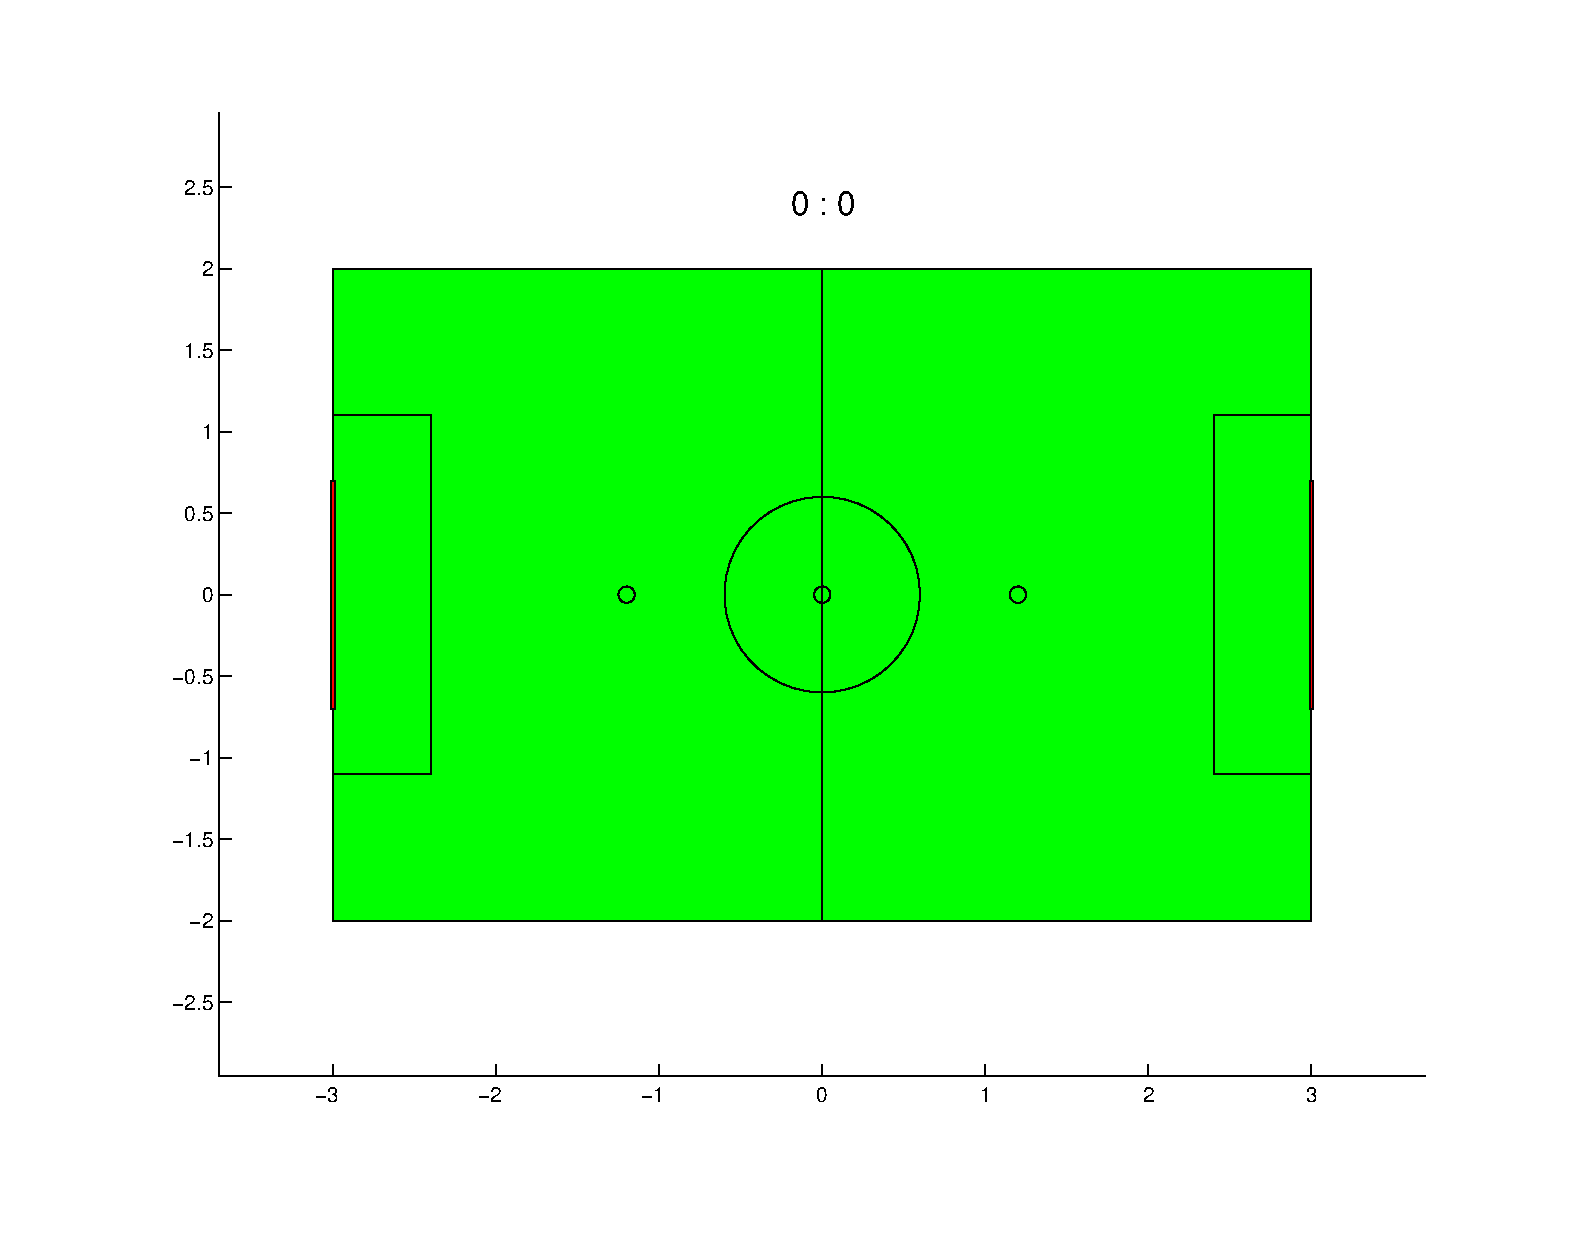
\includegraphics[width=12cm]{./2_Simulation/playing_field}
  	\caption{Playing field after initialization.}
  	\label{KFchart}
\end{figure}


\section{The Robots}

Maybe the most important part of the simulation is the adequate depiction and behaviour of all eight robots. The latter task is split in three components: In a first step the robots are initialized, after that, their new positions on the field, according to their motion equations, are computed and in the end we are adding measurement noise for our filtering task. The initialization of the robots is quite simple. The function {\fontfamily{pcr}\selectfont dummy\_init().m} just creates eight structs with the essential informations for every robot, i.e. its horizontal and vertical position, its direction and its team affiliation. Furthermore the function defines the robot's radius and its maximum possible angular change for one timestep as global variables. In a latter stage of development we dropped the simplification of a global eye and assumed that a location of a robot's position is only possible if it is in the sight of view of at least one other robot. So in the second version {\fontfamily{pcr}\selectfont robot\_init().m} of this function, we additionally defined global variables for the robot's velocity, its distance of sight as well as its angle of sight. Once initialized we use the functions {\fontfamily{pcr}\selectfont dummy\_step(Robot).m} and {\fontfamily{pcr}\selectfont robot\_step(Robot).m} respectively to compute the attributes of all robots for every timestep. The key issue of both functions however is the recalculation of the position, i.e. the motion of the robots

\lstinputlisting[firstline=20, lastline=27]{../Simulation/Merge/dummy_step.m}
\parskip 20pt

Later on this non-linearity of these equations will make it necessary that we use an extended Kalman filter instead of a simple linear one. The addition of process noise and the collision detection of robots also happen in these functions. Up to this point we computed the behaviour of an ideal robot. Since our goal is to filter out the uncertainty of motion of the robot parameters, we artifically have to add some measurement noise which we can filter later on. The functions {\fontfamily{pcr}\selectfont dummy\_measure(Robot).m} and {\fontfamily{pcr}\selectfont robot\_measure(Robot).m} are implemented for that purpose. {\fontfamily{pcr}\selectfont dummy\_measure(Robot).m} simply adds white Gaussian noise to the position and the direction of every robot. Additionally with a certain possibillity there is no measurement at all, so the corresponding parameter is dropped. What we are assuming with this model is, that there is some global eye available which measures the position and direction of every robot with some given resolution. Since this scenario is not realistic in a RoboCup soccer match, because only the robots themselves can gain visual information, we developed the function {\fontfamily{pcr}\selectfont robot\_measure(Robot).m} to solve this problem.



\parskip 10pt

\section{The Ball}



\section{A Random Simulation}


	% -  -  -  -  -  -  -  -  -  -  -  -  -  -  -  -  -  -  -  -  -  -  -  -  -  -  -  -  -  -  -  -  -  -  -  -  -  -  -  -  -  -  -  -  -  -  -  -  -  -  -  -  - %
%-----Chapter 3: Kalman Filtering-------%
\chapter{Kalman Filtering: Theoretical Basics}

\section{Linear Kalman Filter}
There exists a recursive Kalman filter algorithm for discrete time systems.\cite{IntroKF} This ongoing Kalman filter cycle can be divided into two groups of equations
\newline
\begin{enumerate}
	\item Time update equations
	\begin{eqnarray}\label{TupEq}
		%\begin{aligned}
    			\hat{x}_{k}^{-} &= A\hat{x}_{k-1}+Bu_{k-1} \\
    			P_{k}^{-} &= AP_{k-1}A^{T}+Q
  		%\end{aligned}
	\end{eqnarray}
	\item Measurement update equations
	\begin{eqnarray}\label{MupEq}
		%\begin{aligned}
    			K_{k} &= P_{k}^{-}H^{T}(HP_{k}^{-}H^{T}+R)^{-1} \\
    			\hat{x}_{k} &= \hat{x}_{k-1}^{-}+K_{k}(z_{k}-H\hat{x}_{k}^{-}) \\
			P_{k} &= (I-K_{k}H)P_{k}^{-}
  		%\end{aligned}
	\end{eqnarray}
\end{enumerate}

To test this algorithm and to learn something about applying the Kalman filter on linear systems we created an example. A detailed description of the following example can be found in appendix \ref{ExampleKF}. \newline 
We consider a linear, timeinvariant model, given by the following circuit diagram in figure \ref{KFcircuit}.
\begin{figure}[htbp]
	\centering
	\begin{pspicture}(-3,-1)(9,5)
		%nodes
			\pnode(-2,4){A}		\pnode(-2,0){B}		\pnode(8,4){C0}		\pnode(8,0){D}
			\pnode(3,4){A2}		\pnode(3,2){M}		\pnode(3,0){B2}	\pnode(6,4){C2}
			\pnode(6,0){D2}
		%elements
			\coil[intensitylabel=$i_L$,labeloffset=-0.2](A)(A2){$L$}
			\capacitor[tensionlabel=$U_1$,tensionlabeloffset=-1.2,tensionoffset=-0.8,%
					intensitylabel=$i_1$](A2)(M){$C_1$}
			\resistor[tensionlabel=$U_R$,tensionlabeloffset=-1.2,tensionoffset=-0.8](M)(B2){$R$}
			\capacitor[tensionlabel=$U_2$,tensionlabeloffset=-1.2,tensionoffset=-0.8,%
					intensitylabel=$i_2$](C2)(D2){$C_2$}
		%wires
			\wire(B)(D)		\wire(A2)(C0)
			\pscircle[fillstyle=solid](A){0.075}
			\pscircle[fillstyle=solid](B){0.075}
			\pscircle[fillstyle=solid](C0){0.075}
			\pscircle[fillstyle=solid](D){0.075}
		%tension
			\tension(A)(B){$U_{in}$}
			\tension(C0)(D){$U_{out}$}
	\end{pspicture}
    	%\includegraphics[width=12cm]{./3_KalmanFilter/circuit_diagram.jpg}
  	\caption{Example: Linear electrical circuit.}
  	\label{KFcircuit}
\end{figure}
First we added process noise and measurement noise to the system output. The aim is to get an estimation of the noisy output. Therefore we applied the Kalman filter algorithm based on the equations \ref{TupEq}. In the figure \ref{KFchart}, above we can see the input signal and the ideal measurement of the output signal. That ideal measurement includes process noise, which can obviously not be filtered by the Kalman filtering algorithm. Below one can see the noisy measurement on the left side and the filtered output on the right side.
\begin{figure}[htbp]
	\centering
    	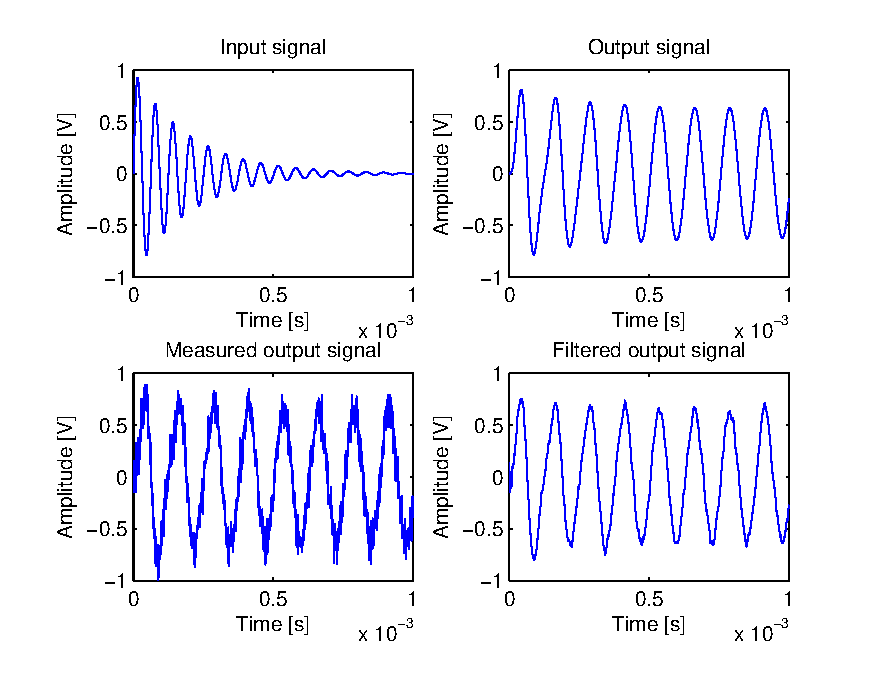
\includegraphics[width=12cm]{./3_KalmanFilterTheory/KFchart.eps}
  	\caption{Example: Input signal, output signal, noisy output, and filtered output.}
  	\label{KFchart}
\end{figure}

\section{Extended Kalman Filter (EKF)}

In the section above we discussed the usage of a Kalman filter on linear systems. Most systems, including the motion equations of our robots, however are nonlinear. Nevertheless linearizing our system around the current estimate still makes our Kalman filter useful and leads to the concept of the extended Kalman filter \cite{IntroKF}. The recursive equations are quite similar to those of the linear Kalman filter
\newline
\begin{enumerate}
	\item Time update equations
	\begin{eqnarray}\label{TupEqEKF}
    			\hat{x}_{k}^- &=& f(\hat{x}_{k-1},u_{k-1},0) \\
    			P_{k}^{-} &=& A_kP_{k-1}A_k^T+W_k Q_{k-1} W_k^T
	\end{eqnarray}
	\item Measurement update equations
	\begin{eqnarray}\label{MupEqEKF}
	%	\begin{aligned}
    			K_{k} &=& P_{k}^- H_k^T(H_k P_k^- H_k^T+V_k R_k V_k^T)^{-1} \\
    			\hat{x}_k &=& \hat{x}_{k-1}^- + K_{k}(z_k - h(\hat{x}_k^-, 0)) \\
			P_k &=& (I-K_k H_k)P_k^-
  	%	\end{aligned}
	\end{eqnarray}
\end{enumerate}

The function \(f(\hat{x}_k,u_k,w_k)\) contains the system's nonlinear dynamics where \(w_k\) represents the current process noise and \(h(\hat{x}_k, v_k)\) denotes the nonlinear state-to-output relationship with the measurement noise \(v_k\). Furthermore the matrices \(A_k\), \(H_k\), \(W_k\) and \(V_k\) are linearizations, i.e. partial drivatives, of their respective functions at time step \(k\)
\newline
%\begin{enumerate}
	\begin{eqnarray}\label{Linearizations}
	%	\begin{aligned}
    			A_{i,j}&= \frac{\partial f_i}{\partial x_j}(\hat{x}_{k-1},u_{k-1},0) \\
    			H_{i,j}&= \frac{\partial h_i}{\partial x_j}(\hat{x}_{k-1},u_{k-1},0) \\
			W_{i,j}&= \frac{\partial f_i}{\partial w_j}(\tilde{x}_k,0) \\
			V_{i,j}&= \frac{\partial h_i}{\partial v_j}(\tilde{x}_k,0)
  	%	\end{aligned}
	\end{eqnarray}
%\end{enumerate}

We dropped the fact that all matrices should have a subscript \(k\) and that they are allowed be different at each time step. Again, before applying the theory to our simulation, we created a generic example of a nonlinear system. Further details can be looked up in section \ref{ExampleEKF}. We did essentially the same as we did for the linear system: We simulated the ideal system, then added process and measurement noise and in the last step checked whether we could get rid of our artifically added measurement noise. The results for a sample run on MATLAB are shown in figure \ref{EKFchart} below

\begin{figure}[htbp]
	\centering
    	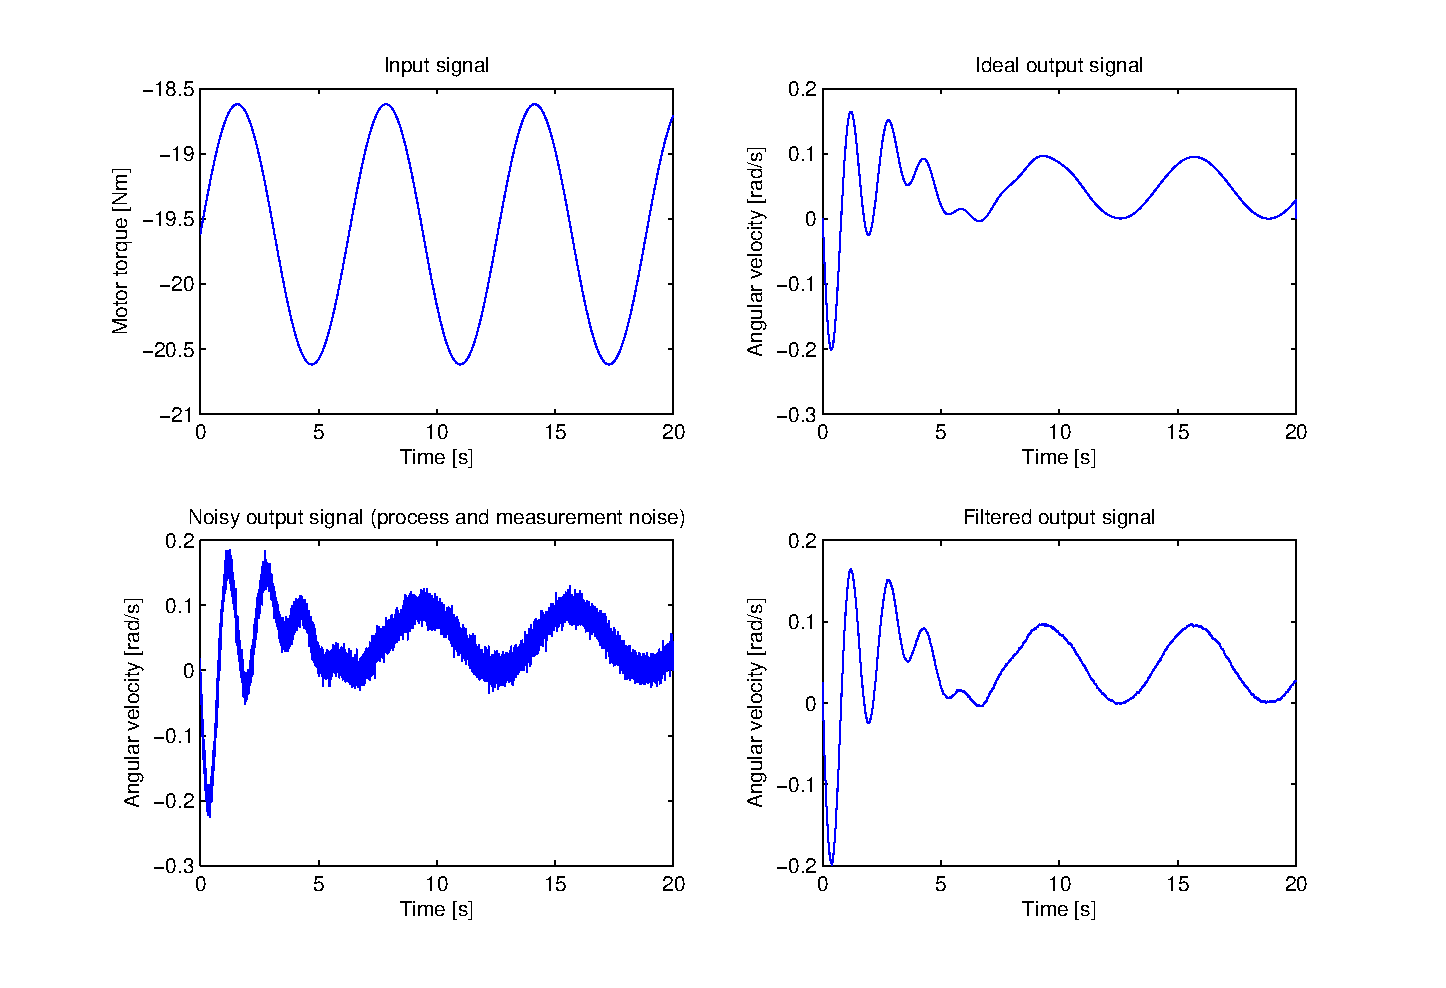
\includegraphics[width=12cm]{./3_KalmanFilterTheory/EKFchart.eps}
  	\caption{Example: Input signal, output signal, noisy output, and filtered output.}
  	\label{EKFchart}
\end{figure}

The two pictures above show the sinusoidal input on the left and the ideal output, i.e. without process and measurement noise, on the right. Thereunder we can see the plots of the noisy signal and the signal after it has been filtered by the extended Kalman filter. We can conclude that the extended Kalman filter too provides an acceptable performance if our measurement noise is not too big.



	
%-----Chapter 4: Estimation-------%
\chapter{Kalman Filtering: Implementation in the MATLAB Environment}

\section{Estimation of the Robots}

As we have seen before, the motion equations of the robots are nonlinear, which makes it necessary to use an extended Kalman filter for the estimation of the robots. The function {\fontfamily{pcr}\selectfont robot\_ekf(robot\_m,robot\_e,m\_values,e\_values,d\_omega,v,P).m} is dedicated for this task. As stated in the theory above, we will need the old estimates and the measurements in order to compute new estimates. Most matrices like the covariance matrices or the Jacobian matrices are the same for all eight robots and hence have to be defined only once. The error covariance \(P\) and the estimator \(K\) on the other side have to be stored for every robot individually, therefore we will use cell arrays for this task. The initialization in MATLAB of these parameters is shown below

\lstinputlisting[firstline=18, lastline=27]{../Simulation/Merge/robot_ekf.m}
\parskip 20pt

In a next step we calculate the Kalman estimate for every robot. In a former version of the function, the two cell arrays {\fontfamily{pcr}\selectfont m\_values} and {\fontfamily{pcr}\selectfont e\_values} contained a history of the last measurements and estimates of the robots. They were used to improve the performance of the extended Kalman filter. The collision detection of former versions of the simulation made it necessary for the filter algorithm to be responsive to large changes of the direction of the robots. Since the Kalman filter itself couldn't handle these rapid changes, we needed a function that indicates that the measurements are much more reliable if there is a huge difference between them and the estimates over a certain space of time. The essential functionality was  to reduce the matrix \(R\), which caused the extended Kalman filter to heaviliy trust the incoming measurements. For this task a history of former measurements and estimates was necessary. But since these problems disappeared with the introduction of collision avoidance, the used methods are obsolete. Therefore we could implement the time update and measurement update equations just as they were stated in the theory. The MATLAB-code below forms the core of the extended Kalman filter for the robots

\lstinputlisting[firstline=48, lastline=62]{../Simulation/Merge/robot_ekf.m}
\parskip 20pt

The prediction of the robot's position and direction can be done for every time step, but the correction is only possible if all measurements are available. This is not the case for example if robots don't get visual information of other robots. With the if-statement we accomodate this fact. So the typical Kalman cycle is only executed if we have measurement on the positions and the direction. Otherwise we drop the measurement update, i.e. our new estimate is simply a simulation of the robot's motion with the former estimates.

\section{Estimation of the Ball}
	
%-----Chapter 5: SensorFusion-------%
\chapter{Sensor Fusion}
In RoboCup every robot works autonomous except a WLAN connection between the teammates. So the whole team can share information to optimize their game.
Through his field of view every robot can bring in some informations about the playing field, other robots and about the ball. Now to optimize the estimation and to exploit the informations from the robots, the team can share this informations in form of a sensor fusion algorithm.
Sensor fusion offers a great opportunity to overcome physical limitations of sensing systems.\cite{IntroSF} 

In the case of RoboCup we need as so called High-level fusion (decision fusion). Methods of decision fusion do not include only the combination of position, edges, corners or lines into a feature map. Rather they imply voting and statistical methods. \cite{IntroSF}

\section{Sensors of the Robots}
The robots comes with a camera with a defined field of view. There are no other sensors or informations with can be used for estimation of the positions. 
There are three types of sensor configuration regarding to sensor fusion. \cite{IntroSF}
\begin{itemize}
	\item Complementary
	\item Competitive
	\item Cooperative
\end{itemize}
In the RoboCup case all the types can occur. The sensor configuration is complementary if a region is  observed by only one robot or camera. And if there are two or more cameras the sensor configuration can be competitive or cooperative.

\section{Principles of Sensor Fusion}
There are several methods 


\section{Dempster-Shafer}


	
%-----Chapter 6: FlawsOutlook-------%
\chapter{Challenges and Outlook}

Several problems which can occur in a real Nao soccer match are covered by our design of the model such as measurement drops, measurement fusion or the fact that inputs of the opposing team are unknown. However there are still practical challenges which we do not encounter in our work. Maybe the most important challenge is the provision of measurements and their related covariances. Up to this point we simply assumed that there is an algorithm which computes the positions and directions of objects on the playing field. We didn't care about the fact whether this can be done in a reliable way or within a reasonable space of time. This task was beyond the scope of this work and certainly could be the subject of another whole group work for the people in the ETHZ RoboCup Team which are occupied with perception.
\parskip 0pt

Other problems arise from the restrictions of our chosen model, for example the assumption that there are only three scenarios under which measurements are gathered. In reality we are probably faced with much more possibilities, that do not only depend on whether a robot sees a landmark or not but also on the actual sight distance to an object or the head angle of a robot. Furthermore the measurement noise may be coloured and not white, so our model would be inaccurate in describing the uncertainty in the given system. Those kind of issues can be summarized as ''lack of detail'', the approximation to reality is not close enough. This can be solved by a better and deeper analysis of the system.

Last but not least there are still several things, that were only partly or not at all considered in our work and which have huge potential for the further localization task. One main aspect here is certainly the practical application of the simulation on the Nao Platform. Not only that it is of course the main goal to have a working estimation and prediction for a real Nao soccer match but also that further improvements of the estimation algorithms will only be possible if they are tested in real environment with real constraints. The modularity of our simulation allows improvements in specific areas concerning estimation. For example the tracking of the ball may be improved too by replacing the extended Kalman filter by a so called particle filter, so switching from deterministic to probabilistic methods. It is also imaginable to have hybrid forms like it is partly done for the extended Kalman filter of the robots (see Ch. 4.1). As a third point one could mention the vast improvements which are possible in estimation if the robots are not acting randomly but if they have a strategy that governs their movements. In terms of localization that would mean that blue robots actively seek getting good measurements and that for example losing the current position of the ball for long periods is not possible anymore. More extensions of the current basic configuration such as better input approximation of enemy robots, the prediction of enemy movements or better handling of discrete events are also thinkable and can have positive effects on the overall performance.



%	
%-----Appendix-------%
\appendix               	% at this point the appendix starts
\chapter{Examples} 
\section{Kalman Filtering of Linear System} \label{ExampleKF} 
\includepdf[pages=-]{./appendix/linear_model.pdf}


	
% Literaturverzeichnis

\addcontentsline{toc}{section}{Literatur}
\begin{thebibliography}{30}

%{\Large\textbf{Books and Articles}}

\bibitem{IntroKF} G. Welch and G. Bishop, ``An Introduction to the Kalman Filter,'' UNC-Chapel Hill, 2006.

\bibitem{RulesRC} RoboCup Technical Committee, ``RoboCup Standard Platform League (Nao) Rule Book,'' RoboCup, 2011.

\bibitem{wwwRoboCup} \texttt{http://www.robocup.org/about-robocup/objective/}\\
Webpage of the RoboCup Organisation, last access:
08.05.2012


\end{thebibliography}
    % includes title literature.tex
\end{document}
